\documentclass[11pt]{article}

\usepackage[utf8]{inputenc}
\usepackage[T1]{fontenc}
\usepackage{graphicx}
\usepackage[linktocpage=true]{hyperref}

\usepackage{mathpazo}

\begin{document}
\begin{titlepage}
	\newcommand{\HRule}{\rule{\linewidth}{0.5mm}}
    \begin{center}
            
    	\textsc{\LARGE Alabama Liquid Snake}\\[0.8cm]
    	\textsc{\Large University of Pretoria}\\[0.5cm]
    	\textsc{\large Epi-Use}\\[0.5cm]
    
    	\HRule\\[0.4cm]
    	
    	{\huge\bfseries Botic - Privacy aware chatbot}\\[0.2cm]
    	
    	{\huge System Requirements Specification}\\[0.2cm]

    	\HRule\\[0.5cm]

	    \textsc{Justin Grenfell} - u16028440 \\[0cm]
	    \textsc{Peter Msimanga} - u13042352 \\[0cm]
	    \textsc{Alicia Mulder} - u14283124 \\[0cm]
	    \textsc{Kyle Gaunt} - u15330967 \\[0cm]
	    \textsc{Lesego Mabe} - u15055214 \\[0cm]
    
    \end{center}
\end{titlepage}
\tableofcontents
\newpage
\section{Introduction}
\begin{flushleft}
A crucial part of any business in today's economic climate is customer service. Those companies that are willing to go the extra mile for their customers are seen as being a cut above the rest. With superior customer service a company can not only bring in new clients, who want an experience that seems to cater to them as an individual, but also successfully retain existing clients by dealing with their issues efficiently and effectively.\\[0.5cm]

In order to do so, there needs to be a system that can record customer feedback and act on it in as soon as possible. In the past, this has been achieved by employing a large number of people around the clock that sit and wait for queries, handle them and then send back the result.\\[0.5cm]

While this works, it is not only inefficient (different employees may respond better or worse than others, employees may not follow protocols, mistakes may be made regularly) but financially costly as well. On top of that, when dealing accounts and queries, customers may inadvertently divulge private information that is not applicable to their case, but may leave them vulnerable should that information become public knowledge.\\[0.5cm]

What if one central system could seamlessly record, interpret and act on the requests of multiple users 24/7 and prevent them from transmitting sensitive data unless absolutely necessary?\\[0.5cm]

\textbf{Botic} is the solution! One system that can not only record user queries, but sanitize their content by filtering out any "data risks" and act on the provided information, returning the appropriate response. Trained on historical data, the system uses artificial intelligence to analyze requests and act accordingly. It scrapes all data before transmission to ensure that no sensitive information is sent to or from the client without clearance from the company's protocols first.\\[0.5cm]

Should the system be unable to find a suitable solution, the request will be handed off to the appropriate customer representative who will then deal with the request. Once that case has been handled, the system will have learned how to deal with future requests of that type and will be able to return a response based on this learning. This will ensure a high level of efficacy for the system as a whole.\\[0.5cm]

Botic will be the front-line for any company that provides customer service feedback facilities or services. The system will reduce the need for a large number of employees for a problem that can be solved using artificial intelligence. It will also improve efficiency and precision when dealing with issues and, due to its constantly learning nature, will become more accurate and able to handle more complex situations as time goes on.\\[0.5cm]
\end{flushleft}

\section{Domain Model}

 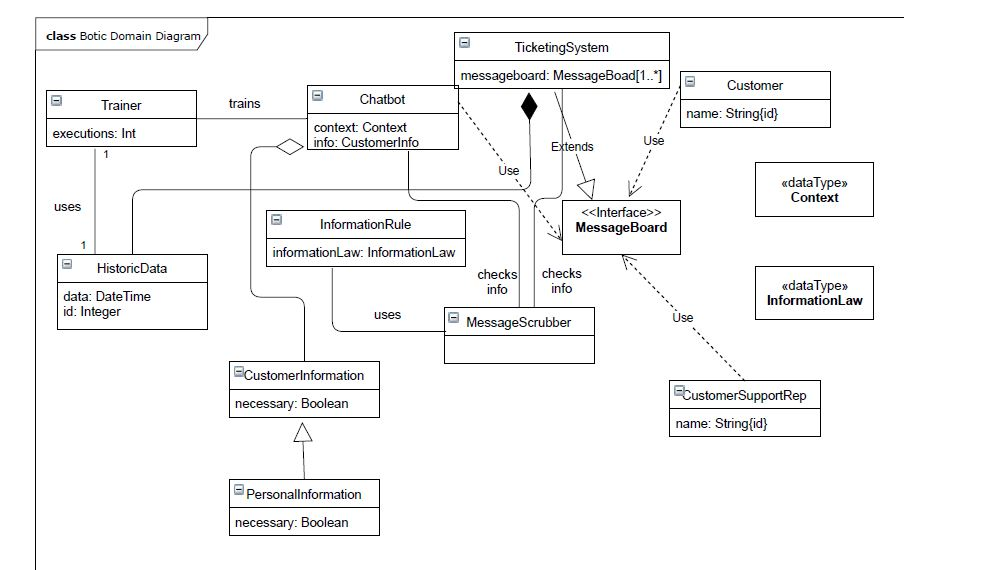
\includegraphics[width=1.0\textwidth]{/images/Botic_Domain_Diagram.jpg}
 
\section{User Characteristics}
\subsection{Customer}
The customer will be submitting information to the system in order to deal with account related queries and, in doing so, may unintentionally submit private/sensitive information that could lead to a breach of confidentiality. Any information sent through by the customer will be sanitized by the system and cleaned up before it is transmitted.
\subsection{Customer Support Representative}
This user will be notified when the automated system is unable to interpret the customer's request and said request will be forwarded. The user will have the ability to respond with the result, whereby the system will sanitize the data once more and send it through to the customer.

\section{Functional Requirements}
\subsection{Information Scraper}
\begin{enumerate}
    \item R1. System must be able to read in a string of information and identify personally identifying information.
    \item R2. System must be able to warn a user if they have entered identifying information. 
    \item R3. System must be able to distinguish between type and severity of identifying information entered.
    \item R4. System front-end must be contained in a portable web component.
\end{enumerate}
 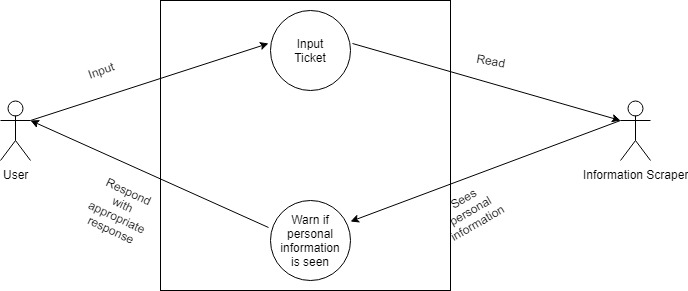
\includegraphics[width=1.0\textwidth]{/images/Information_Scraper_UCD.jpg}
\subsection{AI Chatbot}
\begin{enumerate}
    \item R5. Chatbot must be able to process user input and provide an appropriate response.
    \item R6. Chatbot must be able to read in and recognise a user query and attempt to answer it.
    \begin{enumerate}
        \item R6.1 If the bot is able to recognise user query, it should attempt to answer it.
        \item R6.2 If the bot is unable to recognise user query, it should send the query to a human.
        \item R6.3 The bot should use a text recognition API to understand the input.
    \end{enumerate}
    \item R7. Chatbot must be able to gauge its own ability to respond to a query.
    \item R8. Chatbot must be be able to provide appropriate responses to any query that it can solve.
\end{enumerate}
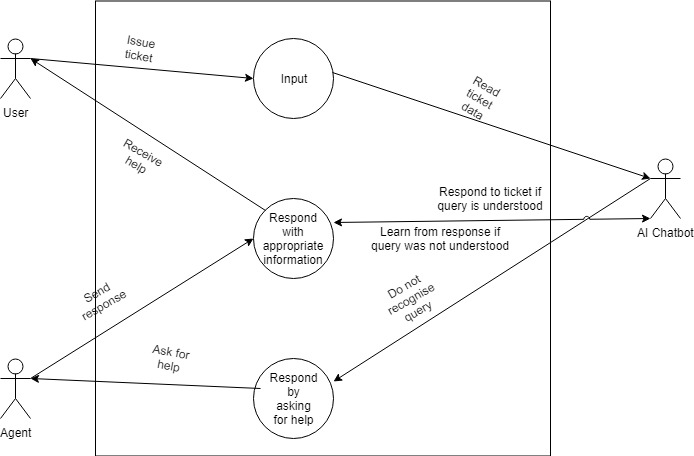
\includegraphics[width=1.0\textwidth]{/images/AI_Chatbot_UCD.jpg}
\subsection{AI Backend}
\begin{enumerate}
    \item R9. Backend must host and server the AI Chatbot and Scraper respectively
    \item R10. Backend must provide the library of responses that the AI has at its disposal.
    \item R11. Backend must train on new and historic information to learn how to identify queries
    \item R12. Backend must train on new and historic information to learn how to identify personally identifying information.
\end{enumerate}
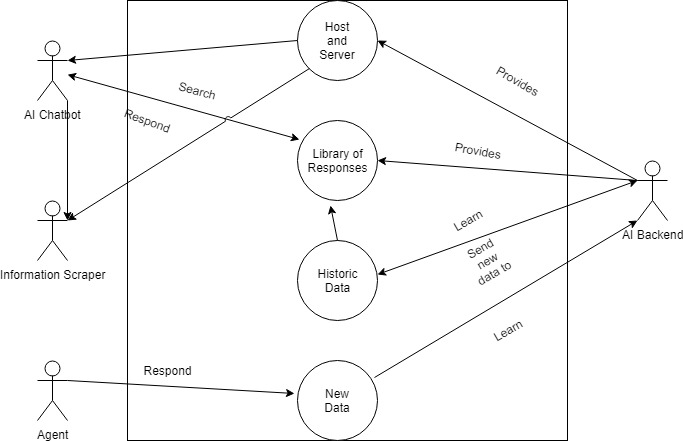
\includegraphics[width=1.0\textwidth]{/images/AI_Backend_UCD.jpg}
\section{Non-Functional Requirements}
The non-functional requirements below will be listed by priority.
\subsection{Availability}
\begin{enumerate}
    \item The system has to have high availability to handle customer queries and issues since it is meant to augment a customer support system, i.e. a ticket system.
    \item The system should be available at least 99 percent of the time, not considering network errors.
\end{enumerate}

\subsection{Performance}
\begin{enumerate}
    \item The system must answer queries as quickly and accurately as it can or divert the query to the relevant customer support specialist in good time. 
\end{enumerate}

\subsection{Scalability}
\begin{enumerate}
    \item The system should be able to scale appropriately to accommodate additional/growing customer queries, especially during peak work hours; it would be useful if the resources scaled down as well during “off peak” hours.
    \item We have chosen to deploy our system to Docker, it is used in part to allow for efficient and easy scaling. More resources can be allocated to our system dynamically - on demand.
\end{enumerate}

\subsection{Maintainability}
\begin{enumerate}
    \item The system structure will be modular to adhere to the concept of low coupling and high cohesion. This would help to make it maintainable since updated systems result in localized changes instead of changes everywhere throughout the system.
    \item We will create a coding standards document which we will also adhere to throughout the system in order to increase readability.
\end{enumerate}

\subsection{Security}
\begin{enumerate}
    \item This pertains to ensuring the [authentication=appropriate word] of customers, to make sure that responses are sent to the correct users.
    \item A log-in system would have to be implemented and private customer information would have to be secured i.e information that would used for authentication purposes like E-mail addresses.
    \item We will be using OAuth for authentication purposes.

\end{enumerate}

\section{Architectural Design}
Our system is an interactive system. We will be using a 3-tier architectural style for the first level of granularity as a result. This architectural tactic/style is in line with making sure that the entire system has highly available. The first layer, has an MVC architecture within.

 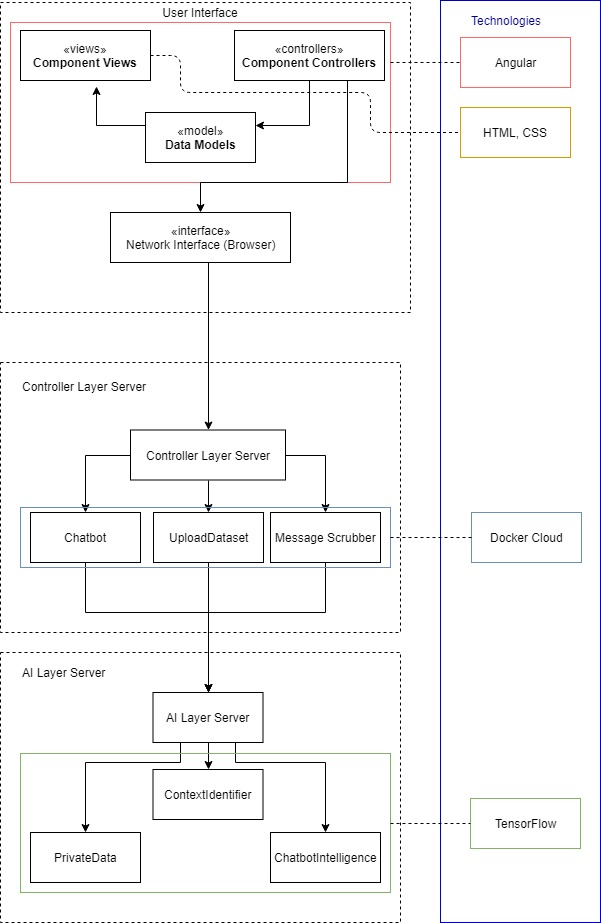
\includegraphics[width=1.0\textwidth]{/images/Botic_Simplified_Architectural_Design.jpg}

\section{Traceability Matrix}
\begin{center}
 \begin{tabular}{||c | c | c | c ||} 
 \hline
  & Information Scraper & AI Chatbot & AI Backend \\
 \hline\hline
 R1 & X &  &  \\
 \hline
 R2 & X &  &  \\
 \hline
 R3 & X &  &  \\
 \hline
 R4 & X &  &  \\
 \hline
 R5 &  & X &  \\
 \hline
 R6 &  & X &  \\
 \hline
 R6.1 &  & X &  \\
 \hline
 R6.2 &  & X &  \\
 \hline
 R6.3 &  & X &  \\
 \hline
 R7 &  & X &  \\
 \hline
 R8 &  & X &  \\
 \hline
 R9 &  &  & X \\
 \hline
 R10 &  &  & X \\
 \hline
 R11 &  &  & X \\
 \hline
 R12 &  &  & X \\
 \hline

\end{tabular}
\end{center}

\end{document}